\chapter{Design}

The design phase translates the requirements identified during system study into a structured representation of the proposed \textbf{AI-LMS} system. It defines the overall architecture, functional interactions, data flow, activity logic, database organization, and user interface layout of the application. The design ensures a clear separation between client presentation, REST API controllers, NoSQL data storage, and Retrieval-Augmented Generation (\textbf{RAG}) vector processing services.

AI-LMS follows a decoupled full-stack architecture in which users interact with a React 18 frontend, authentication and role-based access control (\textbf{RBAC}) are managed via JSON Web Tokens (\textbf{JWT}) and \textbf{Bcrypt}, persistent data is stored in \textbf{MongoDB Atlas}, and vector similarity retrieval is executed using \textbf{Pinecone Vector DB}, \textbf{LangChain}, and \textbf{OpenAI}.

\section{System Architecture}

The system architecture describes the major components of AI-LMS and their interactions. The platform consists of five primary layers: Presentation Layer, Routing \& Security Layer, Application Service Layer, Data Storage Layer, and Vector RAG Subsystem.

The frontend is implemented using React 18, Vite, and Tailwind CSS. React Router manages client-side navigation and enforces protected route guards. The backend is built with Node.js and Express.js, providing 14 modular API controllers secured with JWT Bearer authentication.

Data storage is partitioned between MongoDB Atlas (using Mongoose ODM for entity relationships) and Pinecone Vector DB (for storing 1536-dimensional OpenAI vector embeddings).

The overall architecture of the system is shown in Figure~\ref{fig:systemarchitecture}.

\begin{figure}[H]
    \centering
    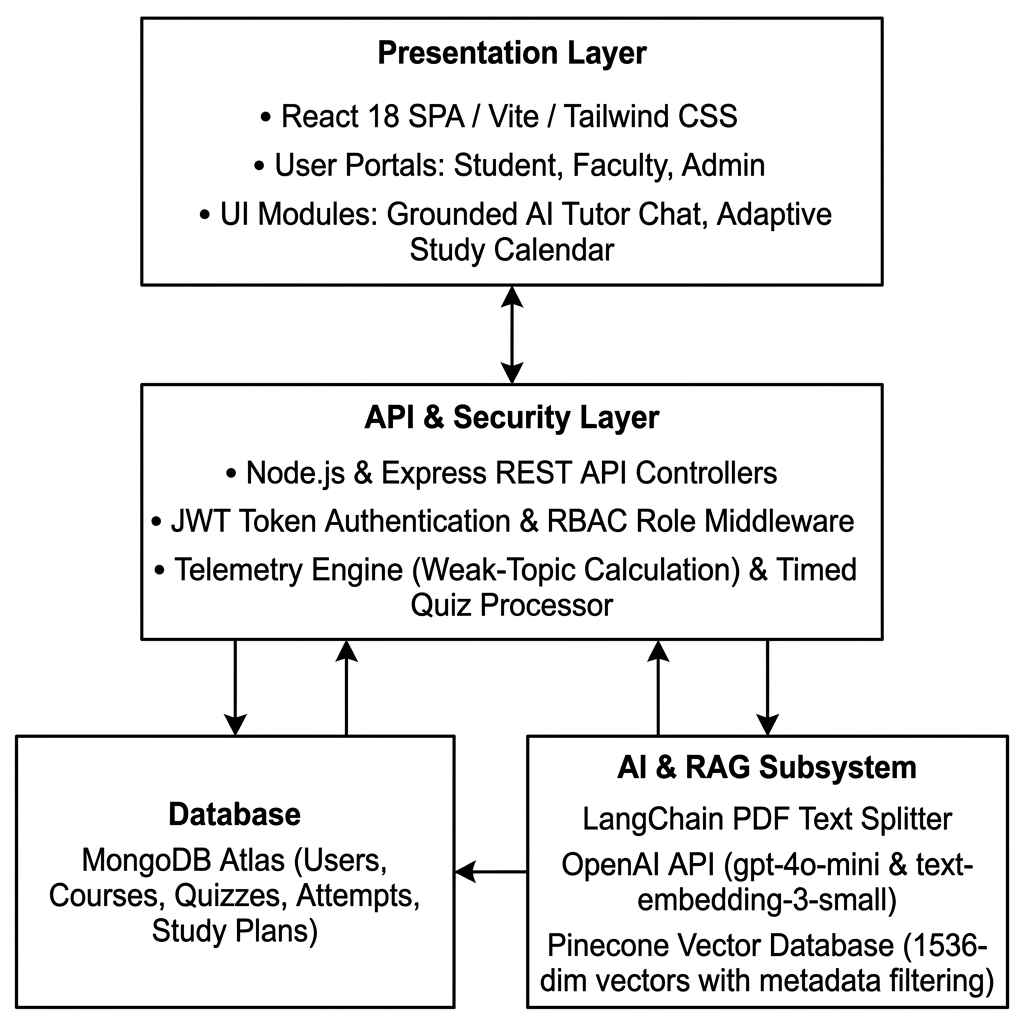
\includegraphics[width=0.9\textwidth]{figures/system_architecture.png}
    \caption{System Architecture of AI-LMS}
    \label{fig:systemarchitecture}
\end{figure}

The major components of the architecture are described below:

\begin{enumerate}
    \item \textbf{Presentation Layer:} Provides the user interface using React components and Tailwind CSS for Students, Faculty, and Administrators.
    
    \item \textbf{Routing \& Security Layer:} Manages navigation between pages and protects authenticated routes using React Router and JWT verification.
    
    \item \textbf{Application Service Layer:} Express.js controllers managing core LMS features, including course building, timed quiz engine, and telemetry tracking.
    
    \item \textbf{Data Storage Layer:} Uses MongoDB Atlas to store users, course structures, quizzes, attempt history, and study plan records.
    
    \item \textbf{Vector RAG Subsystem:} LangChain PDF text chunking, OpenAI embedding generation, and Pinecone vector store executing semantic search with course metadata filters.
\end{enumerate}

\section{Use Case Design}

Use case modeling describes the functional interactions between actors (Student, Faculty, Admin) and the AI-LMS system. The primary actor is the \textbf{Student}, along with \textbf{Faculty} and \textbf{Admin}.

The major use cases identified for the system are:

\begin{itemize}
    \item User Registration \& Role Assignment
    \item User Login \& Token Issuance
    \item View Dashboard \& Enrolled Courses
    \item Upload PDF Lecture Notes (Faculty)
    \item Query Grounded RAG AI Tutor with Page Citations (Student)
    \item Take Timed Quiz \& View Telemetry (Student)
    \item Generate Adaptive AI Study Plan (Student)
    \item Generate AI Quiz Questions (Faculty)
    \item System Governance \& Roles (Admin)
    \item User Logout
\end{itemize}

The use case diagram is shown in Figure~\ref{fig:usecase}.

\begin{figure}[H]
    \centering
    \includegraphics[width=0.9\textwidth]{figures/use_case.png}
    \caption{Use Case Diagram of AI-LMS}
    \label{fig:usecase}
\end{figure}

\subsection{Register}

The Register use case allows a new student, faculty member, or administrator to create an account. The user provides required credentials, which are validated by the system before creating an account with an assigned role.

\subsection{Login}

The Login use case allows registered users to access protected system resources. Authentication credentials are validated against hashed passwords, and upon success, a signed JWT Bearer token is issued.

\subsection{View Dashboard}

The Dashboard provides the primary authenticated interface for each role, displaying course progress, enrolled subjects, telemetry metrics, and quick action links.

\subsection{Query Grounded RAG AI Tutor}

Students submit natural language queries inside enrolled courses. The system vectorizes the query, retrieves matching text chunks from Pinecone, prompts OpenAI \texttt{gpt-4o-mini}, and returns grounded explanations formatted with exact PDF page citations.

\subsection{Take Timed Quiz \& View Telemetry}

Students complete interactive timed quizzes. Upon completion, the telemetry engine evaluates scores, calculates topic mastery, and flags weak knowledge areas ($<60\%$ accuracy).

\subsection{Generate Adaptive AI Study Plan}

Students click to generate a study schedule. The telemetry engine analyzes weak topics and calls OpenAI to construct daily study tasks rendered on an interactive calendar.

\subsection{Upload PDF \& Generate AI Quizzes}

Faculty upload lecture PDFs, which are chunked and indexed into Pinecone. Faculty can also trigger AI automated question generation to build Bloom's taxonomy-aligned quizzes.

\subsection{Logout}

The Logout use case terminates the authenticated session, clears JWT tokens, and revokes access to protected routes until re-authentication.

\section{Data Flow Diagram}

A Data Flow Diagram (DFD) represents the movement of information between users, system processes, and data stores in AI-LMS.

\subsection{Level 0 Data Flow Diagram}

At the context level, AI-LMS is represented as a single system process interacting with users, MongoDB Atlas, and Pinecone Vector DB.

The Level 0 DFD is shown in Figure~\ref{fig:dfdlevel0}.

\begin{figure}[H]
    \centering
    \includegraphics[width=0.85\textwidth]{figures/dfd_level0.png}
    \caption{Level 0 Data Flow Diagram}
    \label{fig:dfdlevel0}
\end{figure}

The student or faculty member provides queries, materials, and quiz attempts through the web interface. The system processes the input and communicates with MongoDB and Pinecone for vector retrieval and telemetry storage.

\subsection{Level 1 Data Flow Diagram}

The Level 1 DFD decomposes the system into six core functional processes: 1.0 Auth \& Role Guard, 2.0 Content Manager, 3.0 RAG Ingestion, 4.0 Grounded RAG Search, 5.0 Quiz Telemetry, and 6.0 AI Study Planner.

The Level 1 DFD is shown in Figure~\ref{fig:dfdlevel1}.

\begin{figure}[H]
    \centering
    \includegraphics[width=0.9\textwidth]{figures/dfd_level1.png}
    \caption{Level 1 Data Flow Diagram}
    \label{fig:dfdlevel1}
\end{figure}

\section{Activity Design}

Activity diagrams represent the operational sequence of control flow within key system features.

\subsection{User Authentication Activity}

The authentication process begins when the user enters credentials. The system validates the inputs against hashed passwords in MongoDB. If valid, a signed JWT Bearer token is issued and the user is redirected to their role-specific dashboard.

The activity flow is shown in Figure~\ref{fig:activitylogin}.

\begin{figure}[H]
    \centering
    \includegraphics[width=0.75\textwidth]{figures/activity_login.png}
    \caption{User Authentication Activity Diagram}
    \label{fig:activitylogin}
\end{figure}

\subsection{RAG Vector Ingestion \& Search Activity}

The RAG process begins when a student submits a natural language question. The system generates a query embedding using OpenAI, searches Pinecone with course metadata filtering, retrieves top matching text chunks, and prompts OpenAI to return a grounded response with page citation badges.

The activity flow is shown in Figure~\ref{fig:activityapplication}.

\begin{figure}[H]
    \centering
    \includegraphics[width=0.75\textwidth]{figures/activity_application.png}
    \caption{RAG Vector Ingestion \& Search Activity Diagram}
    \label{fig:activityapplication}
\end{figure}

\section{Database Design}

AI-LMS uses a hybrid database architecture combining MongoDB Atlas (for relational NoSQL records) and Pinecone (for vector embeddings).

The conceptual database structure used by the application is represented below:

\begin{verbatim}
MongoDB Atlas (Core Relations)     Pinecone Vector Database (Embeddings)
 |                                  |
 +-- users                          +-- course_index
 |    +-- role (student/faculty)         +-- {vectorId} (1536-dim embedding)
 +-- courses                              +-- metadata:
 |    +-- sections / lessons                   +-- courseId
 +-- materials (PDFs)                          +-- pageNumber
 +-- quizzes / questions                       +-- fileTitle
 +-- attempts (telemetry)                      +-- textChunk
 +-- study_plans (tasks)
\end{verbatim}

The database structure is illustrated in Figure~\ref{fig:firestore}.

\begin{figure}[H]
    \centering
    \includegraphics[width=0.8\textwidth]{figures/firestore_schema.png}
    \caption{MongoDB \& Pinecone Database Structure}
    \label{fig:firestore}
\end{figure}

The main fields of core MongoDB collections are described in Table~\ref{tab:applicationfields}.

\begin{table}[H]
\centering
\caption{Core MongoDB Document Schema Fields}
\label{tab:applicationfields}
\begin{tabular}{p{0.25\textwidth} p{0.55\textwidth}}
\toprule
\textbf{Collection} & \textbf{Description \& References} \\
\midrule
Users & Account details, hashed passwords, and role assignment. \\
Courses & Course details, metadata, and instructor references. \\
Lessons / Materials & Lesson sections, video links, and PDF URLs. \\
Quizzes & Timed quiz configurations and question arrays. \\
Attempts & Quiz attempt history, score, and topic accuracy map. \\
StudyPlans & Telemetry weak-topic lists and scheduled study tasks. \\
\bottomrule
\end{tabular}
\end{table}

\section{User Interface Design}

The user interface provides a simple, clean, and accessible environment for accessing course materials, querying the AI Tutor, taking quizzes, and viewing study plans.

\subsection{Student Workspace Interface}

A representation of the student interface layout is shown in Figure~\ref{fig:addapplication}.

\begin{figure}[H]
    \centering
    \includegraphics[width=0.8\textwidth]{figures/add_application.png}
    \caption{Student AI Tutor \& Study Planner Interface}
    \label{fig:addapplication}
\end{figure}

\section{Security Design}

Security is maintained through JWT authentication, role guards, password encryption, and vector metadata isolation.

BcryptJS encrypts user passwords prior to database storage. Stateless JWT Bearer tokens govern API routes. Pinecone vector queries enforce strict `{ courseId }` metadata filtering to ensure vector search retrieves text chunks exclusively from the student's enrolled course.

\section{Design Summary}

The design of AI-LMS defines the architecture, functional interactions, data flow, activity logic, database schemas, and interface structures required for the platform. The design provides a clean separation between presentation, API controllers, NoSQL database, and Pinecone vector stores, providing the foundation for full-stack implementation discussed in Chapter 5.
